\documentclass{sciposter}
\usepackage[utf8]{inputenc}
%\usepackage[brazil]{babel}
\usepackage{multicol}
\usepackage{amsmath, amssymb}
\usepackage{graphicx}
\usepackage{tabularx}
\usepackage{multirow}
\usepackage[dvipsnames]{xcolor}
\usepackage{booktabs}
\usepackage{textcomp} % for registred symbol
\usepackage[linesnumbered,algoruled,longend]{algorithm2e}
\newcommand{\midsepremove}{\aboverulesep = 0mm \belowrulesep = 0mm}
\midsepremove
\newcommand{\midsepdefault}{\aboverulesep = 0.605mm \belowrulesep = 0.984mm}
\midsepdefault

% titulo do trabalho
\font\myfont=cmr12 at 50pt
\title{\myfont Comparing word embedding and computer vision models to predict fMRI data during visual word recognition}

% nome dos autores
\author{Ning Mei$^1$, Usman Sheikh$^1$, Roberto Santana$^2$, David Soto$^1$}


% nome e endereço da Instituição
\institute{1. Basque Center on Cognition, Brain, and Language, San Sebastian, Spain\\ 2. University of Basque Country, Spain}

% e-mail dos autores (em ordem)
\email{{semsociaty, d.soto.b}{(@gmail.com})}

% exibe os logos (esquerda e direita) 
\leftlogo[1.2]{bcbl.jpeg}
\rightlogo[0.9]{qr-code.png}

%%%%%%%%%%%%%%%%%%%%%%%%%%%%%%%%%%%%%%%%%%%%%%%%%%%%%%%%%%%%%%%%%%%%%%%%%%%%%%%%
%%% Begin of Document

\begin{document}


\conference{{\bf CCN-2019}, Conference of Cognitive Computational Neuroscience at Berlin, Germany}

\maketitle

\newcommand{\mycaption}{%
\ifx \@captype \@undefined \@latex@error {\noexpand \caption outside float}\@ehd \expandafter \@gobble \else \refstepcounter \@captype \expandafter \@firstofone \fi {\@dblarg {\@caption \@captype }}%
}%

%%% Begin of Multicols-Enviroment
\begin{multicols}{3}

%%% Abstract
% \begin{abstract}
% Abstract.
% \end{abstract}

%%% Introduction
\section{Introduction}

\begin{enumerate}
    \large
    \item Semantic memory is the cognitive function that holds and retrieves language related information \cite{binder2009a}.
    \item fMRI-based classification studies \cite{bauerneural} have shown that the semantic category of both pictures and words can be decoded from multivoxel patterns in different brain regions of the so-called semantic network \cite{binder2009a}. \textcolor{red}{\textbf{Encoding models}} further enable us to understand the type of information that is represented in brain activity during language processing tasks and define how the brain derives a cognitive map of meaning \cite{naselaris2011a,felsen2006a}.
    \item However, how the brain representation of conceptual knowledge varies as a function of internal processing goals and strategies remains unclear.
    \item Word embedding algorithms (i.e. Word2Vec-2013 \cite{mikolov2013a}) provide a way to characterize the geometry of semantic spaces. 
    \item Computer vision models (i.e. deep convolutional neural network \cite{lecun1998gradient} also reveal the structural organization of meaning in the ventral visual pathway \cite{simonyan2014very}.
    \item To examine the properties of the semantic representations in the brain during word recognition, we tested different encoding models based on \textcolor{red}{\textbf{word embedding models}} and \textcolor{red}{\textbf{computer vision models}}.
\end{enumerate}

\section{Experiment}

\begin{enumerate}
    \large
    \item 27 participants.
    \item 18 living and 18 non-living \textbf{words}. Note: \textcolor{red}{no image of objects was shown}
    \item The experiment was comprised of 8 fMRI runs.  Each trial began with a fixation period of 250 ms followed by a blank screen of 500 ms (see Figure \ref{fig1}) and then by the target visual word which was displayed for \textbf{1 s}.
    \item Depending on session instructions (shallow or deep processing), the participants were asked  to either read and attend to the word (\textbf{shallow process condition}), or mentally simulate the properties associated with the word (e.g. its shape, its color etc., \textbf{deep process condition}).
    \item Following  a prior meta-analysis \cite{binder2009a}, 15 left-lateralized areas were pre-specified and included regions withing inferior parietal lobe, lateral temporal, ventromedial temporal lobe including fusiform gyrus and parahippocampal gyrus, dorsomedial prefrontal cortex, inferior frontal gyrus, ventromedial prefrontal cortex, posterior cingulate gyrus and anterior temporal lobe.
    \item Word embedding models includes \textcolor{brown}{Word2Vec-2013} \cite{mikolov2013a}, \textcolor{RubineRed}{GloVe} \cite{Pennnigton2014a}, and \textcolor{red}{Fast Text} \cite{bojanowski2016a}
    \item Computer vision models includes \textcolor{blue}{VGG-19} \cite{simonyan2014very}, \textcolor{yellow}{DenseNet121} \cite{howard2017mobilenets}, and \textcolor{green}{MobileNetV2} \cite{huang2017densely}
\end{enumerate}

\begin{figure}
    \centering
    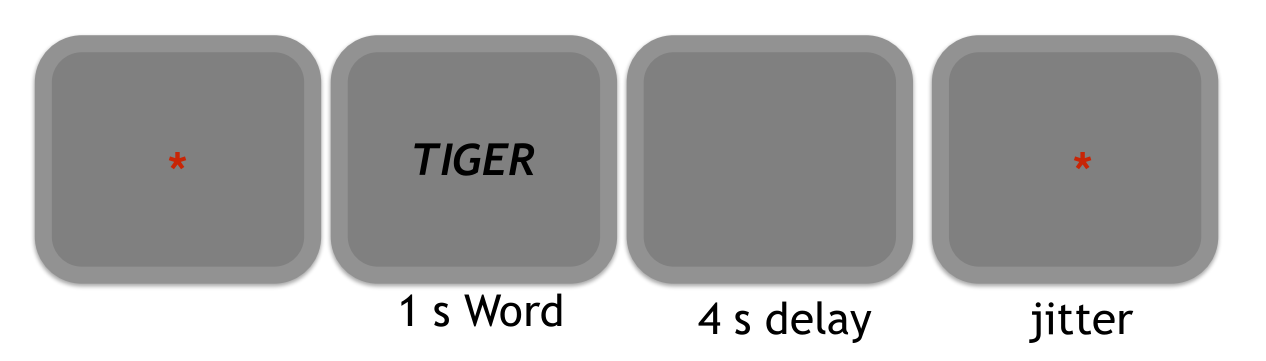
\includegraphics[width=1.\linewidth]{paradigm.png}
    \caption{Experiment Paradigm}
    \label{fig1}
\end{figure}

\begin{figure}
    \centering
    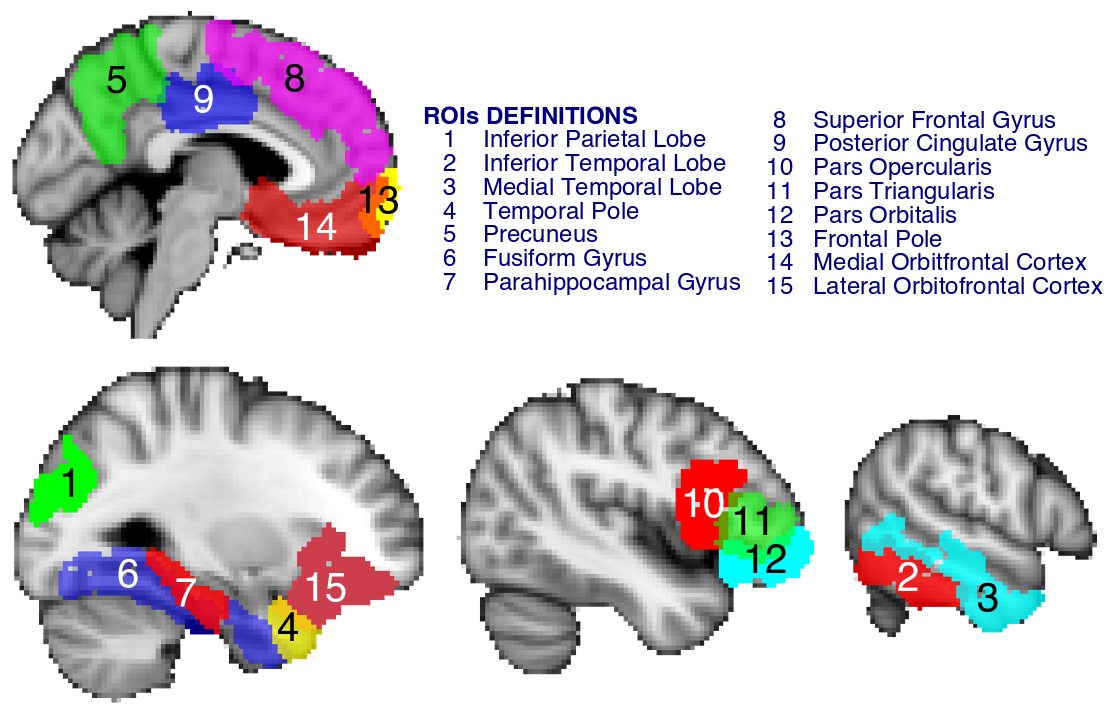
\includegraphics[width=1.\linewidth]{Fig2.png}
    \caption{Region of Interests}
    \label{fig2}
\end{figure}

\section{Encoding Model}

\begin{enumerate}
    \large
    \item An encoding model predicts the brain activity patterns using a set of features that are (non)linearly transformed from the stimuli \cite{Diedrichsenkriegeskorte2017a, KriegeskorteDouglas2018a}. In order to map the sensory stimuli to the brain activity, the encoding model reconstructs/predicts the brain activity patterns by utilizing a given set of feature/representational spaces extracted from the stimuli \cite{naselariskay2015a}.
    \item We hypothesized image-like features were more likely to be mentally represented during the ‘deep information processing’ condition relative to the ‘shallow processing‘ condition. Therefore, besides three word-embedding models (Word2Vec-2013, GloVe, and FastText), we selected three computer vision models (VGG-19, MobileNetV2, and DenseNet121) to extract features from images corresponding to the words we used in the experiment.
\end{enumerate}

\section{Results, ***: p $<$ 0.001, **: p $<$ 0.01, *: p $<$ 0.05, n.s.: not significant}
\begin{figure}
    \centering
    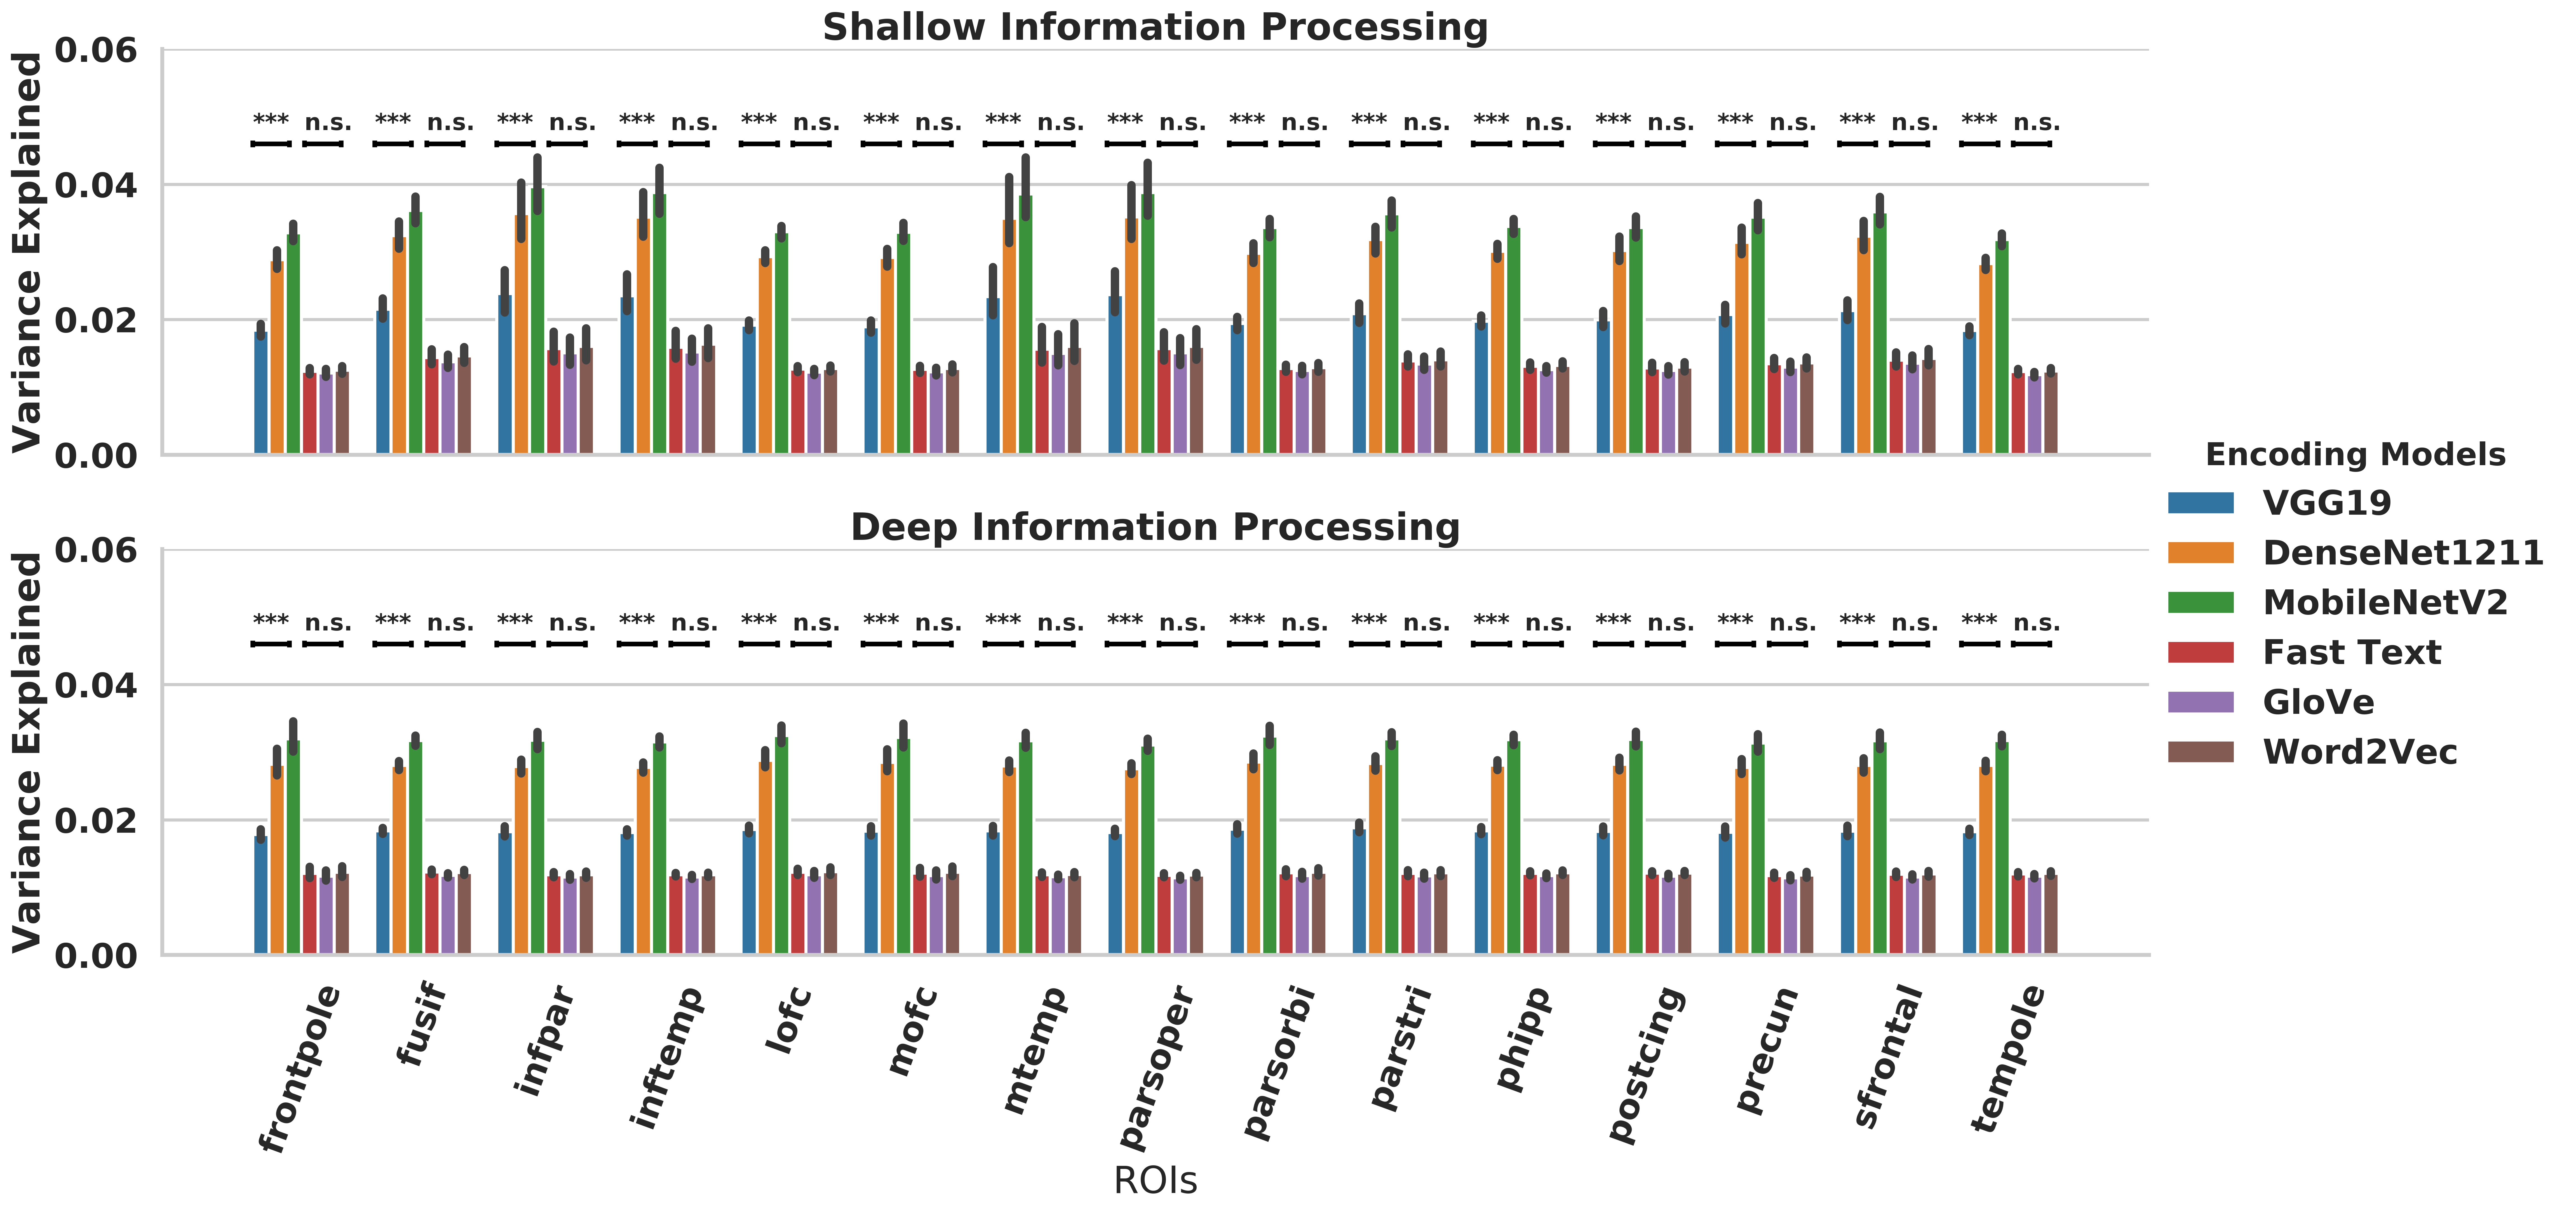
\includegraphics[width=1.07\linewidth]{fig5.png}
    \caption{Average Variance Explained}
    \label{fig3}
\end{figure}

\large
We subtracted variance explained of each word embedding model from each computer vision model. And then we compared each pair of differences against zero. The multiple comparison was corrected with either shallow or deep process condition by FDR Benjamini-Hochberg procedure. 

\begin{figure}
    \centering
    
\includegraphics[width=1.07\linewidth]{fig6.png}
    \caption{Difference of Variance Explained by the Computer Vision Model and Word Embedded Model}
    \label{fig4}
\end{figure}

%\section{Comparison the Differences between Computer Vision Models and Word Embedding Models between Shallow and Deep Process}

\large
We then averaged the difference between each computer vision and word embedding model, for each subject and for both shallow or deep processing conditions, and compared these across subjects. Multiple comparison correction was performed across the ROIs using FDR Benjamini-Hochberg procedure. 

\begin{figure}
    \centering
    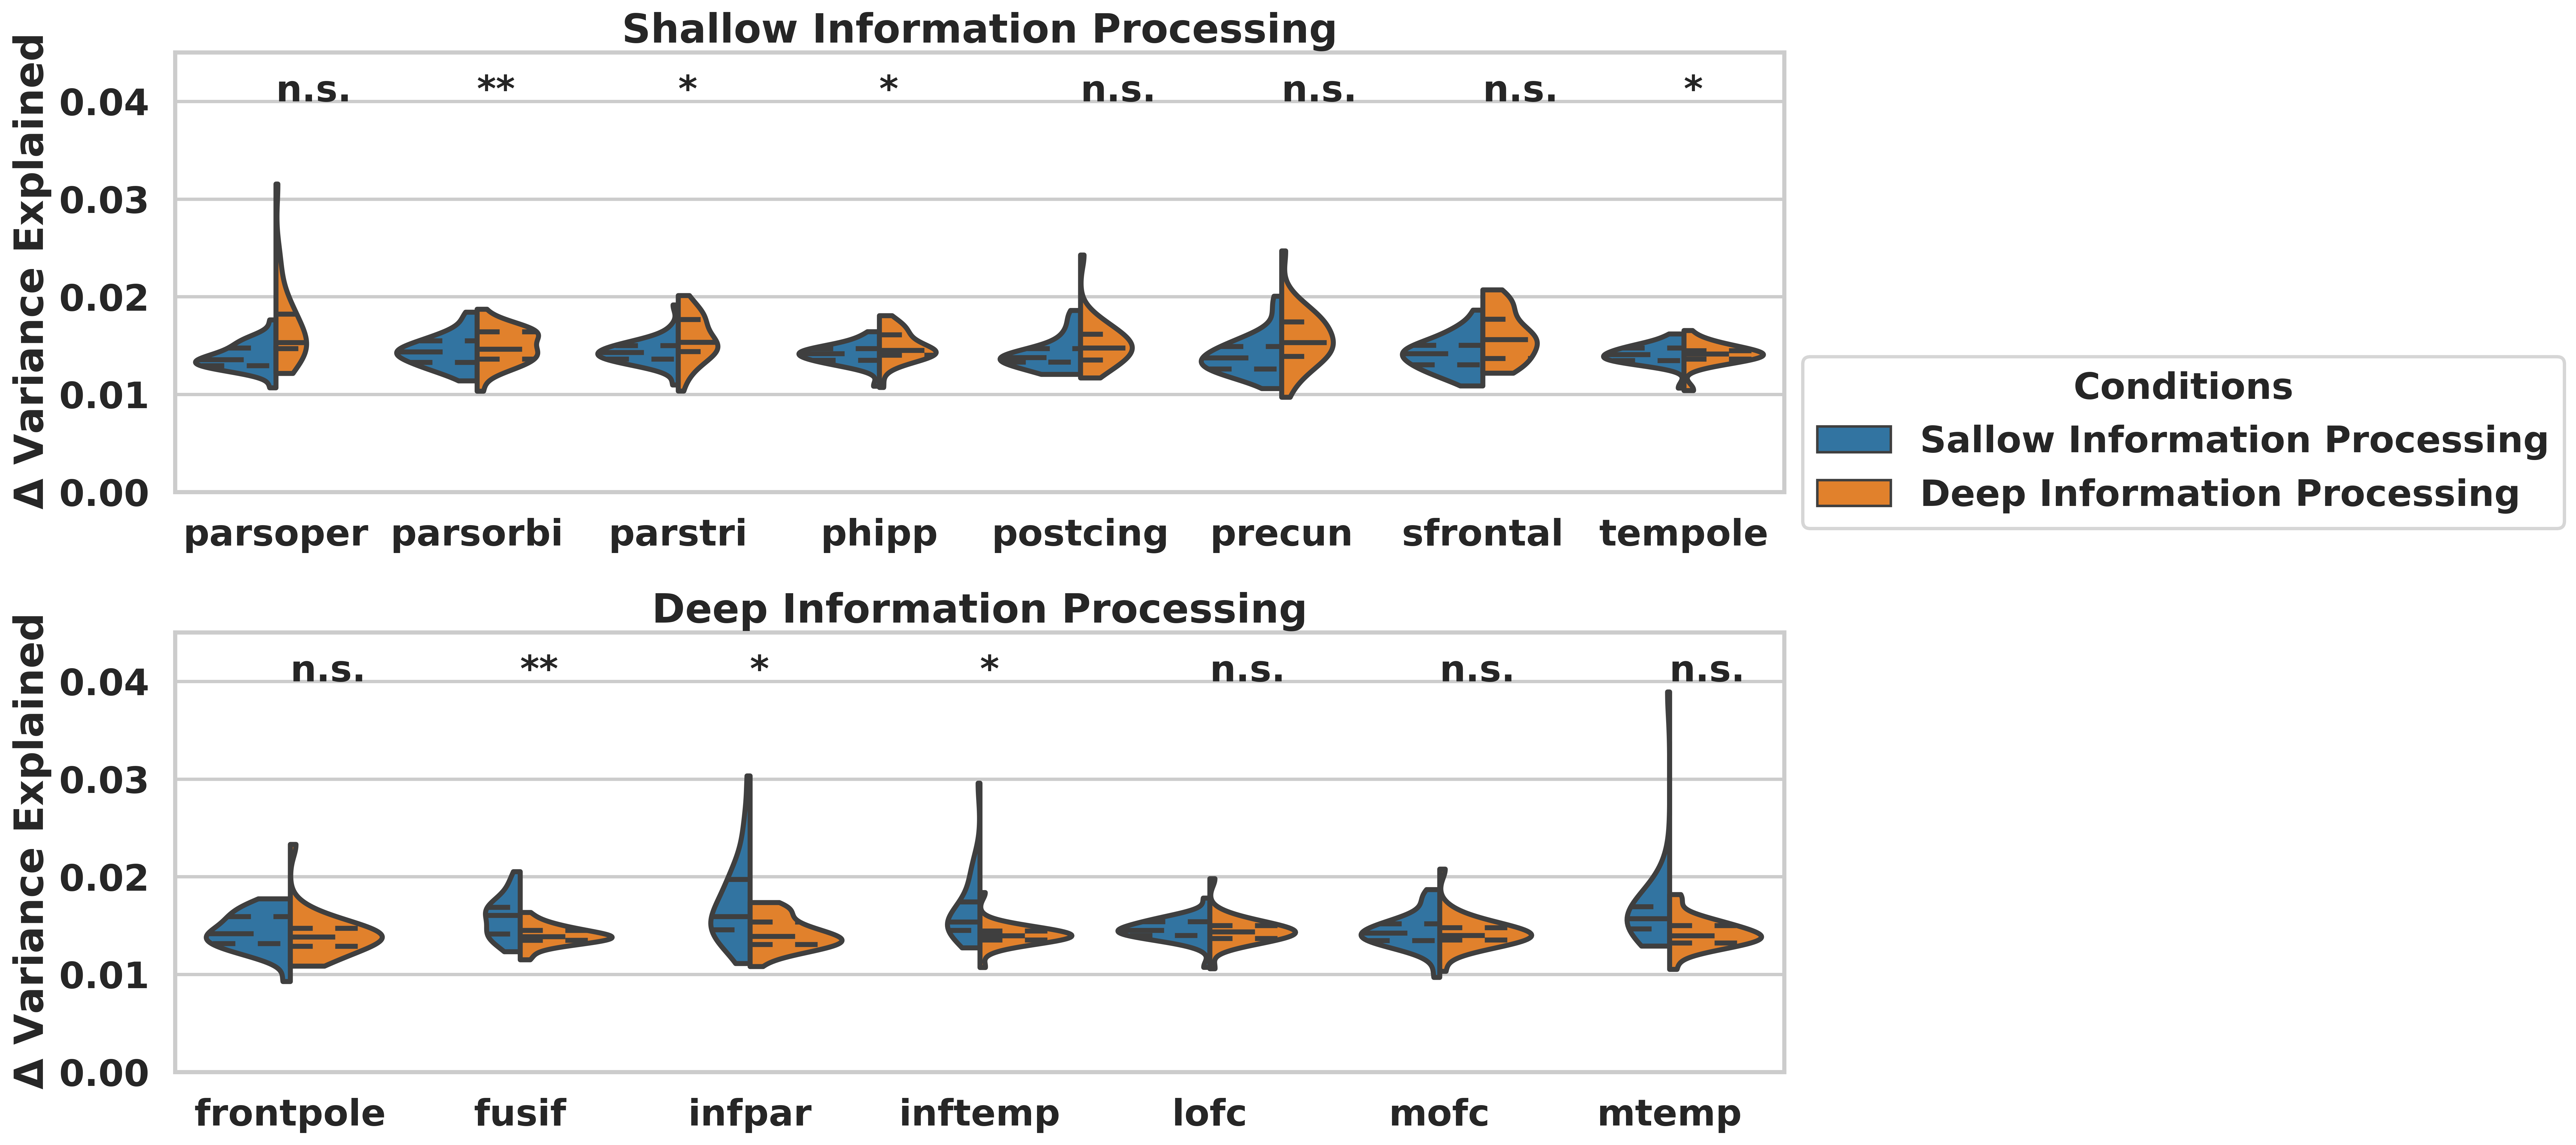
\includegraphics[width=1.\linewidth]{fig7.png}
    \caption{Difference of Computer Vision Models and Word Embedding Models contrast between shallow and deep process}
    \label{fig5}
\end{figure}

\section{Conclusion and Limitation}

\begin{enumerate}
    \large
    \item Computer vision models outperformed word embedding models in explaining brain responses during semantic processing tasks. This pattern occurred independently of the task demand (shallow vs deep process the words). 
    \item Computer vision models predicted more variance in visual areas such as the fusiform during deep information process condition, which is consistent with participants accessing to visual representations during mental simulation of the concept. 
    \item The abstract representations from the embedding layer of computer vision models provide a better "semantic" model of how the brain encodes word meanings \cite{vogel2007semantic}.
    \item The representations of the computer vision models are much larger than those of the word embedding models (1000$^+$ v.s. 300). This is due to the fact that none of the models was fine-tuned before applied to the dataset.
\end{enumerate}

%%% References

\bibliographystyle{plain}
{\tiny \bibliography{bib/references}}
  
\section{Acknowledgements}
\tiny
D.S. and N.M. acknowledges support from the Spanish Ministry of Economy and Competitiveness, through the 'Severo Ochoa' Programme for Centres/Units of Excellence in R \& D (SEV-2015-490) and project grants PSI2016-76443-P from MINECO and PI-2017-25 from the Basque Government. R. S. acknowledges support by the Basque Government (ELKARTEK programs), and Spanish Ministry of Economy and Competitiveness MINECO (project TIN2016-78365-R).

\end{multicols}

\end{document}
